\documentclass{sig-alternate}
\usepackage{graphicx}
\usepackage{subfigure}
\usepackage[ruled,vlined,boxed]{algorithm2e}
\usepackage{fancyvrb}
\usepackage{balance}
\usepackage{epsfig}
\usepackage{times}

\begin{document}

\title{Contours Polygon Validation \\
       Documentation Report}

\numberofauthors{1}

\author{
Bryan Katigbak$^{1}$\\
\\
\begin{tabular}{c}
$^1$Center for Comprehensive Informatics, Emory University \\
%$^2$Center for Comprehensive Informatics, Emory University \\
%$^3$Center for Comprehensive Informatics, Emory University \\
\end{tabular}
\\
\\
\\
}

\maketitle
\begin{abstract}
Processing of image mark-ups as result of various algorithm generates several invalid polygon structures. Odd shapes and unpredictable patterns are not an issue as long as the resulting contour constitute a valid polygon.

The primary purpose is to come up with a right tool to normalize these contours to be able to successfully loaded into DB2 database for further analysis and processing.

Goals:\\
  - eliminate intersections\\
  - resolve loops\\
  - remove unnecessary coordinates\\
  - simplify

Invalid cases can be categories or identified by giving descriptive names such as dangling, rings (or loops), T-intersections ,self-intersection and tangent intersections.

The bottom line of all this irregularities is the presence of intersection. Ultimately, to address this is to smoothen or untangle these knots by either removal or unnecessary coordinate or to introduce (insert) new coordinate as part of the resulting contour. Splitting (clipping) of contours into component simple polygon is also a possibility. By including all resulting simple polygon increase the covered area by the original contour rather that simply removing the significant area of the contours.

\end{abstract}

%\begin{figure}
% \centering
%\framebox[3.1in][c]{
% 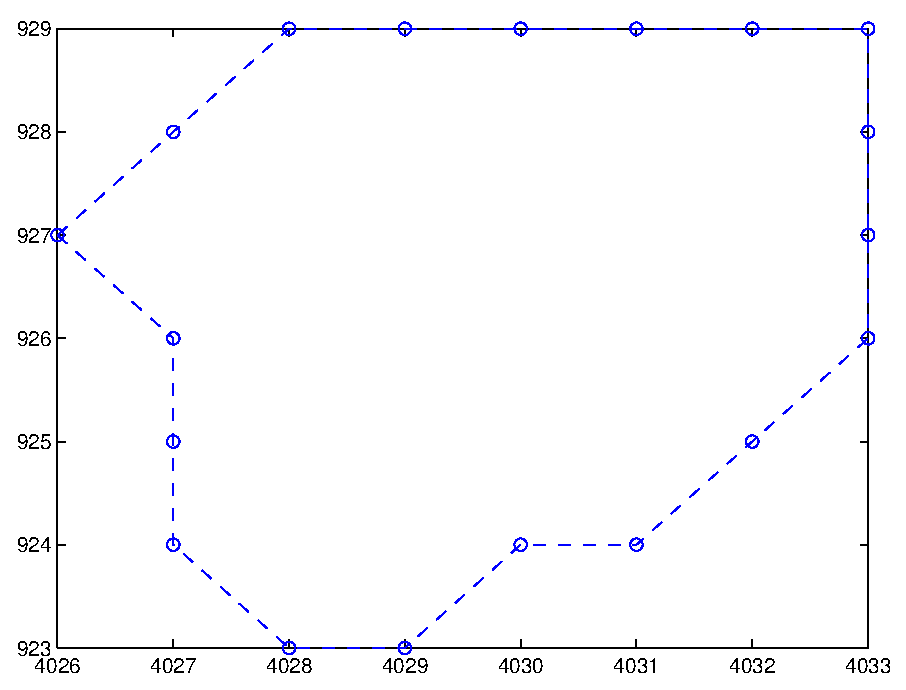
\includegraphics[width=3in]{untitled}
%}
%  \caption{Test dummy image}

% \label{fig:testimage}
%\end{figure}


%\begin{figure}
%\centering
%\includegraphics[width=3in]{dangling1}
%\label{fig:dangling1}
%\end{figure}


%I have a test image as show in Figure \ref{fig:testimage}.



\section{Contour Simplification}
In this process unnecessary coordinates are removed from the contour sequence. Unnecessary coordinates must not affect the general layout (shape) of the resulting contour. By doing this processing effort will drop significantly. Factors that determine the simplification of contours are: coordinate directional sequence, collinear, duplicate  and gradient conditions.
\subsection{Clockwise Direction}
Sequence of coordinates does not dictates the overall appearance of the polygon. Either clockwise or counter clockwise same structure will be formed. However, it is difficult to analyse individual coordinates in terms of linear iteration. Change in direction implies intersection, thus the only way to resolve this is to split the contour right at the point of intersection. 
The newly formed sequence is required to reverse the order to follow the standard clockwise order. 
\subsection{Collinear Points}
These are coordinates in between in a given line segment in such a way when ignored (deleted) will not affect the orientation of the resulting segment  and in turn the resulting polygon. One can say that these could be a set of points lying on a straight line bounded by 2 end points, any coordinates in between is basically unnecessary.
\subsection{Duplicate Points}
Redundant by itself  means unnecessary, therefore it duplicates must be removed.
\subsection{Gradient}
Determines the degree of significance in  contours simplification. Based on my observation DB2 for some instances sharp (or narrow)  angle is considered self-intersection. By raising the gradient variable such condition will be ignored resulting to the deletion of the problematic coordinate.

\section{Multiple Polygon}
Contours forming multiple linked polygons will be clipped to form individual simple polygon. Segment intersections forming an enclosed area triggers a polygon split up. Complex set of polygon contours will form disintegrated simple polygons.

\section{Exceptions}
\subsection{Segment Intersection}
In some instances segment intersection arises from forced polygon closure step. Since last coordinate is forced to be equal to the first coordinate, thus it is possible that the segment  that will connects between  first (or last) and last -1 will intersect the original contour.
In the case intersecting segments positioned between 1 or 2 coordinates apart, currently algorithms provided by Boost and Clipper Libraries failed to handle these.

To rectify this issue, a recursive iteration inspecting the contours for segment intersection in both clock wise and counter clockwise manner. The coordinate that causing the intersection will be deleted from the contour. This change in the contour might trigger yet another intersection therefore this procedure is repeated until no such intersection is detected.

Intersection point sometimes is not present in the given contour. But it does not means that there is no possibility of segment intersection. All we need to do is to find to that specific coordinate using the formula described in the next section.

\section{WorkFlow}
\begin{figure}
 \centering
%\framebox[3in]{
 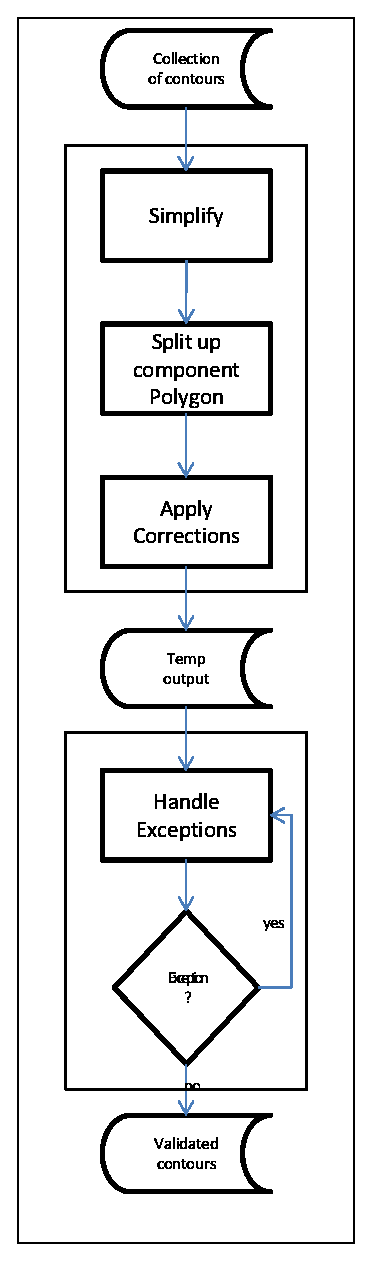
\includegraphics[height=6in]{workflow.eps}
%}
 \caption{workflow diagram}

 \label{fig:workflow diagram}
\end{figure}


\section{Working Equations}

Slope of a straight line.
\begin{equation}
    m = \frac{(y_1 - y_0)}{(x_1 - x_0)}
\end{equation}

Straight-line equations "slope-intercept" form is utilized to verify if a given point is a subset of a given segment. Whereby, m represent the slope and b as the y-intercept.
\begin{equation}
    y = mx + b
\end{equation}

Intersection Point Distance Formula.
Let $t$ represents the variable distance from point $x_0y_0$ to $x_1y_1$ in given line segment. If the the condition holds $0<= t >= 1$
for a given point, we can say that it is in the bounds of the given line segment. Intersection coordinate must lie in between the bounds of the pairing subjected line segments. In this equation $t_P$ represents segment 1 with respect to pair of xy coordinate $x_0,y_0$ and $x_1,y_1$ and likewise with pairing segment Q.
\begin{equation}
    t_P =
    \frac {((Q_{y1}-Q_{y0})*(P_{x1}-P_{x0})-(Q_{x1}-Q_{x0})*(P_{y1}-P_{y0}))} {((Q_{x1}-Q_{x0})*(P_{y0}-Q_{y0})-(Q_{y1}-Q_{y0})*(P_{x0}-Q_{x0}))}
\end{equation}
Cross Product equation derived from pairing segments.


\section{Include Libraries}
Clipper Lib \\
http://www.angusj.com/delphi/clipper/documentation/Docs/\_Body.htm
Simplifypolygon() - this function is responsible for analysing if a given contour represents a simple polygon. If multiple enclosures are identified, it will return a array of individual simple polygon.

Boost Geometry Lib \\
http://www.boost.org/doc/libs/1\_49\_0/libs/geometry/doc/html/index.html
simplify() - this rectifies conditions such as collinear and duplicate coordinates.
correct() - affix closure endpoints if necessary and ensures that the sequence of coordinates is in clock-wise manner, which is not so much important for simple polygons.

%\cite{wang2011evaluation}

\section{Related Readings}
Below are the excerpt from Oracle User Guide and Reference web site that can be used as a guide for polygon contour validation:
For geometry consistency, the function checks for the following, as appropriate for the specific geometry type:

Polygons have at least four points, which includes the point that closes the polygon. (The last point is the same as the first.)

Polygons are not self-crossing.

No two vertices on a line or polygon are the same.

Polygons are oriented correctly. (Exterior ring boundaries must be oriented counterclockwise, and interior ring boundaries must be oriented clockwise.)

An interior polygon ring touches the exterior polygon ring at no more than one point.

If two or more interior polygon rings are in an exterior polygon ring, the interior polygon rings touch at no more than one point.

Line strings have at least two points (plus the start and end points).

\section{sample cases}
Contour Simplification (Collinear and Duplicate)\\
Under simple case scenario, assuming that there are no intersection, loops or any irregularities. Standard simplification process eliminates collinear and duplicates. As already mention earlier, eliminating these case are only nice to have because it improves efficiency by reducing unnecessary items in a given data. The following frames show the effect of this process.

\begin{figure}
% \centering
%\framebox[3in]{
 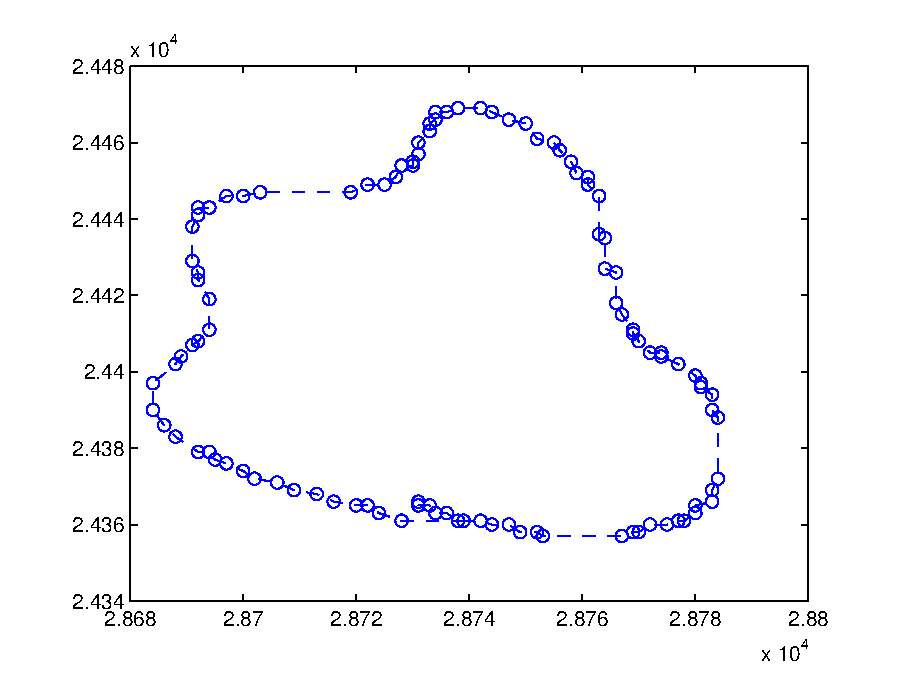
\includegraphics[height=2.5in]{simplify0.eps}
 \includegraphics[height=2.5in]{simplify1.eps}
%}
 \caption{Dangling}

 \label{fig:Dangling}
\end{figure}

Dangling \\

This case can be described as with dangling tail ends under a relatively small contour scenario.
\begin{verbatim}
1510,4098 1510,4094 1520,4094 1523,4094 1525,4092  
\end{verbatim}
\begin{verbatim}
1530,4094 1542,4088 1540,4083 1532,4086 1527,4084  
\end{verbatim}  
\begin{verbatim}
1527,4083 1524,4086 1519,4087 1514,4085 1510,4088
\end{verbatim}
\begin{verbatim}
 1515,4094 1510,4094 
\end{verbatim}
 
Analysing this given contour will give us 3 sets of contours. Taking a closer look at point(1510,4094) it is a intersection point in two instances. Although the first instance will be deleted since it is collinear, still the fact exist that it is a intersection point. We also say that the number of resulting components are equivalent number of intersection points plus 1.
 
Simplifying by setting the max\_dist parameter determines a significant role in overall appearance of the resulting polygon. For instance, point(1527,4083) with max\_dist of 2 shown in third frame. Which means any 
coordinates within the vicinity of 2 units of pixels will be ignored. For illustration purposes second frame has a max\_dist of 0 to show the effect.\\
 
\begin{figure}
% \centering
%\framebox[3in]{
 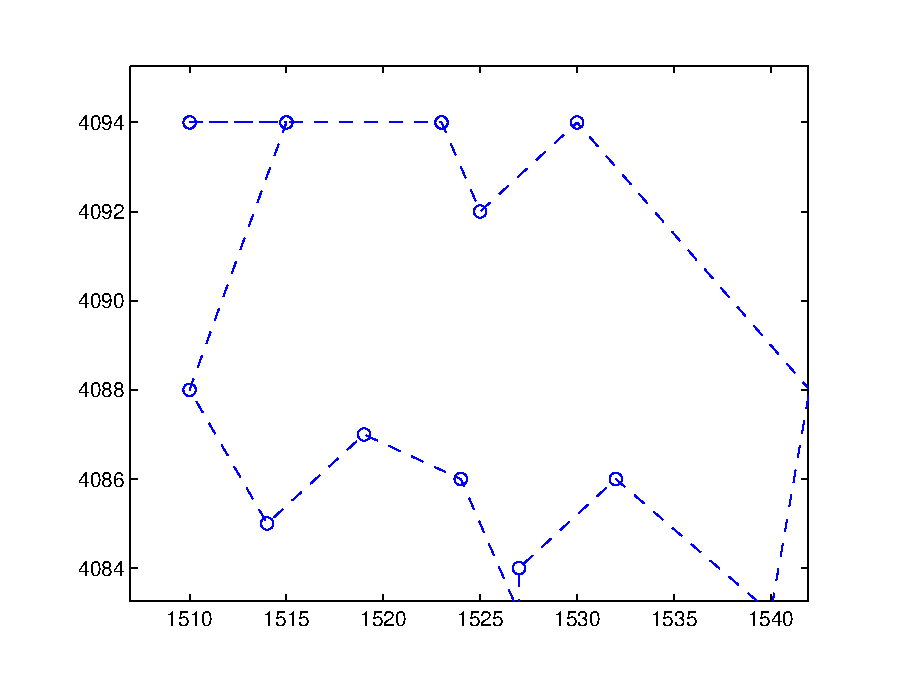
\includegraphics[height=2.5in]{dangle_orig.eps}
 \includegraphics[height=2.5in]{dangle_dist0.eps}
 \includegraphics[height=2.5in]{dangle_dist2.eps}
%}
 \caption{Dangling}

 \label{fig:Dangling}
\end{figure}

Multi-polygon \\

This case is characterized with large contour. But upon simplification a dramatic reduction of significant points. But despite the deletion of these coordinates the overall appearance and structure is kept intact. 
If you zoom in the frames of the following figure you will notice that the original structure was split into two. The lower half seems still a compound polygon but in reality it is not, due to the size of this sample white space was not clearly evident on this one.
The importance of being able to extract all possible polygon on a given contour allows us to gather as much as possible valid polygons as opposed to assuming only one from a given contour. But still this is not a fool proof method since it is also possible that indeed that the whole structure is single whole object.\\  

\begin{figure}
% \centering
%\framebox[3in]{
 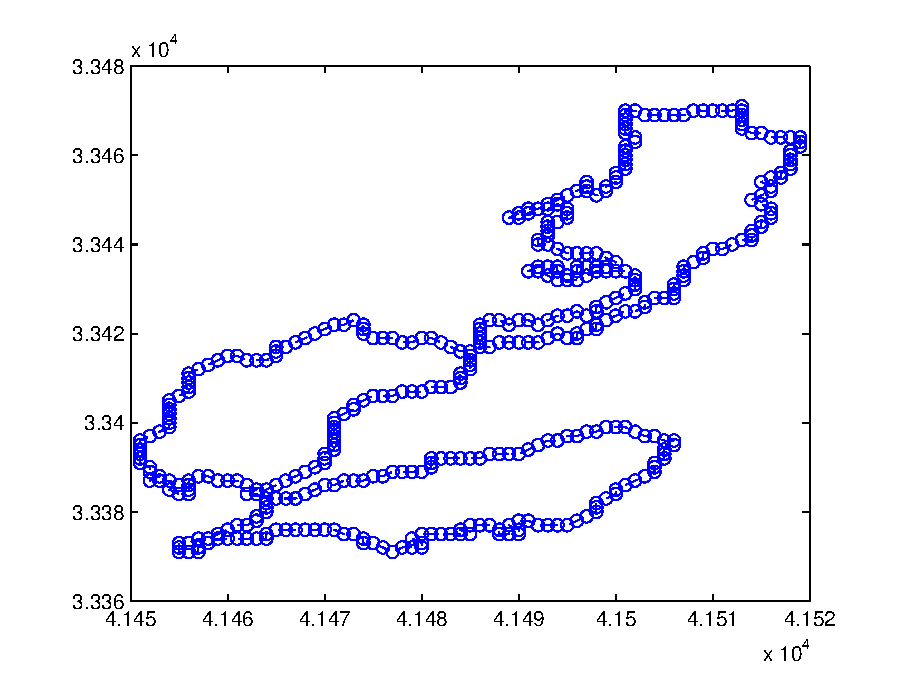
\includegraphics[height=2.5in]{split0.eps}
 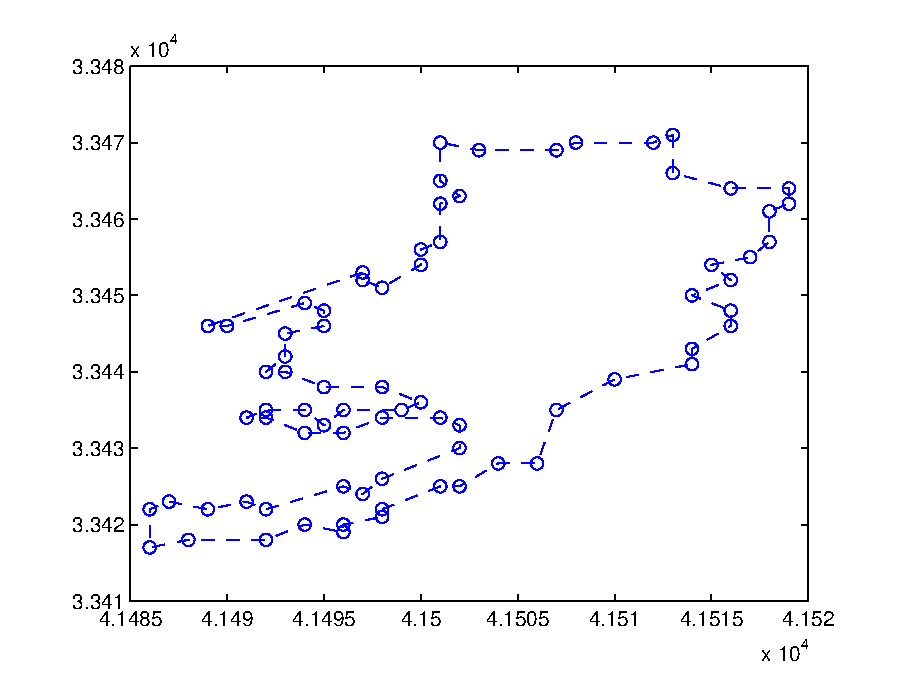
\includegraphics[height=2.5in]{split1.eps}
 \includegraphics[height=2.5in]{split2.eps}
%}
 \caption{Multi-polygon}

 \label{fig:Multi-polygon}
\end{figure}

Self-Intersect\\

Open ended contour can be fixed as simple as connecting both ends together. But this is not a  straight forward solution in actual processing. Self-intersection is possible to arise thus making it challenging and one might say creating another conflict rather that resolving it. 
To rectify this scenario, all offending coordinates starting from the outer towards the middle of the contour will be subjected to self-intersection test. If such case is encounter, that particular coordinate will be discarded until the entire contour validated.
The following figure shows that in this case both ends where trimmed down. Then the new end points emerges as the coordinates closer to each other and the segment formed is not in any way intersecting any other segment of the polygon.

\begin{figure}
% \centering
%\framebox[3in]{
 \includegraphics[height=2.5in]{open_self_intersect.eps}
 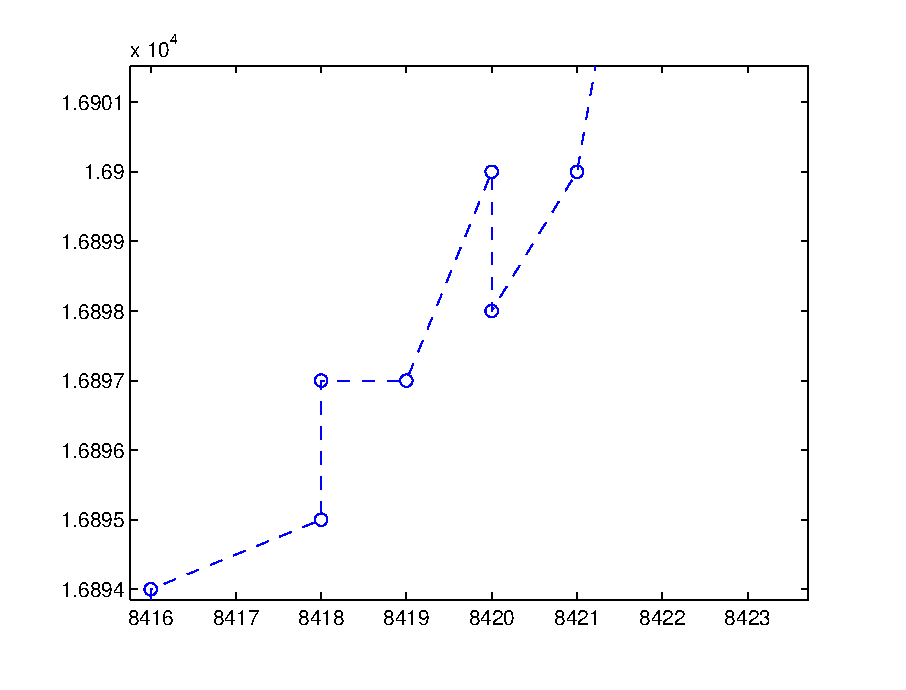
\includegraphics[height=2.5in]{open_self_intersect_resolve.eps}
%}
 \caption{Open Ended}

 \label{fig:Open ended}
\end{figure}


 \bibliographystyle{alpha}
 \bibliography{pais}

\end{document}
